% Options for packages loaded elsewhere
\PassOptionsToPackage{unicode}{hyperref}
\PassOptionsToPackage{hyphens}{url}
%
\documentclass[
]{article}
\usepackage{amsmath,amssymb}
\usepackage{iftex}
\ifPDFTeX
  \usepackage[T1]{fontenc}
  \usepackage[utf8]{inputenc}
  \usepackage{textcomp} % provide euro and other symbols
\else % if luatex or xetex
  \usepackage{unicode-math} % this also loads fontspec
  \defaultfontfeatures{Scale=MatchLowercase}
  \defaultfontfeatures[\rmfamily]{Ligatures=TeX,Scale=1}
\fi
\usepackage{lmodern}
\ifPDFTeX\else
  % xetex/luatex font selection
\fi
% Use upquote if available, for straight quotes in verbatim environments
\IfFileExists{upquote.sty}{\usepackage{upquote}}{}
\IfFileExists{microtype.sty}{% use microtype if available
  \usepackage[]{microtype}
  \UseMicrotypeSet[protrusion]{basicmath} % disable protrusion for tt fonts
}{}
\makeatletter
\@ifundefined{KOMAClassName}{% if non-KOMA class
  \IfFileExists{parskip.sty}{%
    \usepackage{parskip}
  }{% else
    \setlength{\parindent}{0pt}
    \setlength{\parskip}{6pt plus 2pt minus 1pt}}
}{% if KOMA class
  \KOMAoptions{parskip=half}}
\makeatother
\usepackage{xcolor}
\usepackage[margin=1in]{geometry}
\usepackage{color}
\usepackage{fancyvrb}
\newcommand{\VerbBar}{|}
\newcommand{\VERB}{\Verb[commandchars=\\\{\}]}
\DefineVerbatimEnvironment{Highlighting}{Verbatim}{commandchars=\\\{\}}
% Add ',fontsize=\small' for more characters per line
\usepackage{framed}
\definecolor{shadecolor}{RGB}{248,248,248}
\newenvironment{Shaded}{\begin{snugshade}}{\end{snugshade}}
\newcommand{\AlertTok}[1]{\textcolor[rgb]{0.94,0.16,0.16}{#1}}
\newcommand{\AnnotationTok}[1]{\textcolor[rgb]{0.56,0.35,0.01}{\textbf{\textit{#1}}}}
\newcommand{\AttributeTok}[1]{\textcolor[rgb]{0.13,0.29,0.53}{#1}}
\newcommand{\BaseNTok}[1]{\textcolor[rgb]{0.00,0.00,0.81}{#1}}
\newcommand{\BuiltInTok}[1]{#1}
\newcommand{\CharTok}[1]{\textcolor[rgb]{0.31,0.60,0.02}{#1}}
\newcommand{\CommentTok}[1]{\textcolor[rgb]{0.56,0.35,0.01}{\textit{#1}}}
\newcommand{\CommentVarTok}[1]{\textcolor[rgb]{0.56,0.35,0.01}{\textbf{\textit{#1}}}}
\newcommand{\ConstantTok}[1]{\textcolor[rgb]{0.56,0.35,0.01}{#1}}
\newcommand{\ControlFlowTok}[1]{\textcolor[rgb]{0.13,0.29,0.53}{\textbf{#1}}}
\newcommand{\DataTypeTok}[1]{\textcolor[rgb]{0.13,0.29,0.53}{#1}}
\newcommand{\DecValTok}[1]{\textcolor[rgb]{0.00,0.00,0.81}{#1}}
\newcommand{\DocumentationTok}[1]{\textcolor[rgb]{0.56,0.35,0.01}{\textbf{\textit{#1}}}}
\newcommand{\ErrorTok}[1]{\textcolor[rgb]{0.64,0.00,0.00}{\textbf{#1}}}
\newcommand{\ExtensionTok}[1]{#1}
\newcommand{\FloatTok}[1]{\textcolor[rgb]{0.00,0.00,0.81}{#1}}
\newcommand{\FunctionTok}[1]{\textcolor[rgb]{0.13,0.29,0.53}{\textbf{#1}}}
\newcommand{\ImportTok}[1]{#1}
\newcommand{\InformationTok}[1]{\textcolor[rgb]{0.56,0.35,0.01}{\textbf{\textit{#1}}}}
\newcommand{\KeywordTok}[1]{\textcolor[rgb]{0.13,0.29,0.53}{\textbf{#1}}}
\newcommand{\NormalTok}[1]{#1}
\newcommand{\OperatorTok}[1]{\textcolor[rgb]{0.81,0.36,0.00}{\textbf{#1}}}
\newcommand{\OtherTok}[1]{\textcolor[rgb]{0.56,0.35,0.01}{#1}}
\newcommand{\PreprocessorTok}[1]{\textcolor[rgb]{0.56,0.35,0.01}{\textit{#1}}}
\newcommand{\RegionMarkerTok}[1]{#1}
\newcommand{\SpecialCharTok}[1]{\textcolor[rgb]{0.81,0.36,0.00}{\textbf{#1}}}
\newcommand{\SpecialStringTok}[1]{\textcolor[rgb]{0.31,0.60,0.02}{#1}}
\newcommand{\StringTok}[1]{\textcolor[rgb]{0.31,0.60,0.02}{#1}}
\newcommand{\VariableTok}[1]{\textcolor[rgb]{0.00,0.00,0.00}{#1}}
\newcommand{\VerbatimStringTok}[1]{\textcolor[rgb]{0.31,0.60,0.02}{#1}}
\newcommand{\WarningTok}[1]{\textcolor[rgb]{0.56,0.35,0.01}{\textbf{\textit{#1}}}}
\usepackage{graphicx}
\makeatletter
\def\maxwidth{\ifdim\Gin@nat@width>\linewidth\linewidth\else\Gin@nat@width\fi}
\def\maxheight{\ifdim\Gin@nat@height>\textheight\textheight\else\Gin@nat@height\fi}
\makeatother
% Scale images if necessary, so that they will not overflow the page
% margins by default, and it is still possible to overwrite the defaults
% using explicit options in \includegraphics[width, height, ...]{}
\setkeys{Gin}{width=\maxwidth,height=\maxheight,keepaspectratio}
% Set default figure placement to htbp
\makeatletter
\def\fps@figure{htbp}
\makeatother
\setlength{\emergencystretch}{3em} % prevent overfull lines
\providecommand{\tightlist}{%
  \setlength{\itemsep}{0pt}\setlength{\parskip}{0pt}}
\setcounter{secnumdepth}{-\maxdimen} % remove section numbering
\ifLuaTeX
  \usepackage{selnolig}  % disable illegal ligatures
\fi
\IfFileExists{bookmark.sty}{\usepackage{bookmark}}{\usepackage{hyperref}}
\IfFileExists{xurl.sty}{\usepackage{xurl}}{} % add URL line breaks if available
\urlstyle{same}
\hypersetup{
  hidelinks,
  pdfcreator={LaTeX via pandoc}}

\author{}
\date{\vspace{-2.5em}}

\begin{document}

\hypertarget{simple-linear-regression-confidence-and-prediction-intervals}{%
\section{Simple Linear Regression: Confidence and Prediction
intervals}\label{simple-linear-regression-confidence-and-prediction-intervals}}

Earlier we have introduced the simple linear regression as a basic
statistical model for the relationship between two random variables. We
used the least square method for estimating the regression parameters.

Recall that the simple linear regression model for \(Y\) on \(x\) is
\[Y=\beta_0+\beta_1 x+\epsilon\] where

\(Y\) : the dependent or response variable

\(x\) : the independent or predictor variable, assumed known

\(\beta_0,\beta_1\) : the regression parameters, the intercept and slope
of the regression line

\(\epsilon\) : the random regression error around the line.

and the regression equation for a set of \(n\) data points is
\(\hat{y}=b_0+b_1\;x\), where
\[b_1=\frac{S_{xy}}{S_{xx}}=\frac{\sum (x_i-\bar{x})(y_i-\bar{y})}{\sum (x_i-\bar{x})^2}\]
and \[b_0=\bar{y}-b_1\; \bar{x}\] where \(b_0\) is called the
\textbf{y-intercept} and \(b_1\) is called the \textbf{slope}.

\(~\)

\textbf{Under the simple linear regression assumptions}, the residual
standard error \(s_e\) is an unbiased estimate for the error standard
deviation \(\sigma\), where

\[s_e=\sqrt{\frac{SSE}{n-2}}=\sqrt{\frac{\sum(y_i-\hat{y}_i)^2}{n-2}} \]
\(s_e\) indicates how much, on average, the observed values of the
response variable differ from the predicated values of the response
variable.

\(~\)

Below we will see how we can use these least square estimates for
prediction. First, we will consider the inference for the conditional
mean of the response variable \(y\) given a particular value of the
independent variable \(x\), let us call this particular value \(x^*\).
Next we will see how to predicting the value of the response variable
\(Y\) for a given value of the independent variable \(x^*\). These
confidence and predictive intervals, to be valid, the usual four simple
regression assumptions must hold.

\hypertarget{inference-for-the-regression-line-eleftyxright}{%
\subsection{\texorpdfstring{Inference for the regression line
\(E\left[Y|x^*\right]\)}{Inference for the regression line E\textbackslash left{[}Y\textbar x\^{}*\textbackslash right{]}}}\label{inference-for-the-regression-line-eleftyxright}}

Suppose we are interested in the value of the regression line at a new
point \(x^*\). Let's denote the unknown true value of the regression
line at \(x=x^*\) as \(\mu^*\). From the form of the regression line
equation we have

\[\mu^*=\mu_{Y|x^*}=E\left[Y|x^*\right]=\beta_0+\beta_1 x^*\]

but \(\beta_0\) and \(\beta_1\) are unknown. We can use the least square
regression equation to estimate the unknown true value of the regression
line, so we have

\[\hat{\mu}^*=b_0+b_1 x^*=\hat{y}^*\]

This is simply a point estimate for the regression line. However, in
statistics, point estimate is often not enough, and we need to express
our uncertainty about this point estimate, and one way to do so is via
confidence interval.

A \(100(1-\alpha)\%\) confidence interval for the conditional mean
\(\mu^*\) is
\[\hat{y}^*\pm t_{\alpha/2}\;\cdot s_e\;\sqrt{\frac{1}{n}+\frac{(x^*-\bar{x})^2}{S_{xx}}}\]
where \(S_{xx}=\sum_{i=1}^{n} (x_i-\bar{x})^2\), and \(t_{\alpha/2}\) is
the \(\alpha/2\) critical value from the t-distribution with \(df=n-2\).

\begin{center}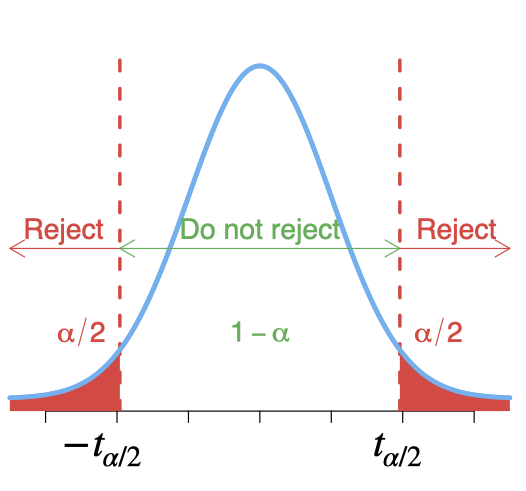
\includegraphics[width=0.35\linewidth,height=0.35\textheight]{figures/Ttest2} \end{center}

\hypertarget{inference-for-the-response-variable-y-for-a-given-xx}{%
\subsection{\texorpdfstring{Inference for the response variable \(Y\)
for a given
\(x=x^*\)}{Inference for the response variable Y for a given x=x\^{}*}}\label{inference-for-the-response-variable-y-for-a-given-xx}}

Suppose now we are interested in predicting the value of \(Y^*\) if we
have a new observation at \(x^*\).

At \(x=x^*\), the value of \(Y^*\) is unknown and given by
\[Y^*=\beta_0+\beta_1 x^*+\epsilon\] where but \(\beta_0\), \(\beta_1\)
and \(\epsilon\) are unknown. We will use \(\hat{y}^*=b_0+b_1\;x^*\) as
a basis for our prediction.

\(~\)

A \(100(1-\alpha)\%\) prediction interval for \(Y^*\) at \(x=x^*\) is

\[\hat{y}^* \pm t_{\alpha/2}\;\cdot s_e\;\sqrt{1+\frac{1}{n}+\frac{(x^*-\bar{x})^2}{S_{xx}}}\]
The extra '1' under the square root sign, we have here to account for
the extra variability of a single observation about the mean.

Note: we construct a confidence interval for a parameter of the
population, which is the conditional mean in this case, while we
construct a prediction interval for a single value.

\hypertarget{example-used-cars-cont.}{%
\subsection{Example: used cars (cont.)}\label{example-used-cars-cont.}}

\textbf{Estimate the mean price of all 3-year-old cars, \(E[Y|x=3]\):}

\[\hat{\mu}^*=195.47-20.26 (3)= 134.69=\hat{y}^*\]

\begin{center}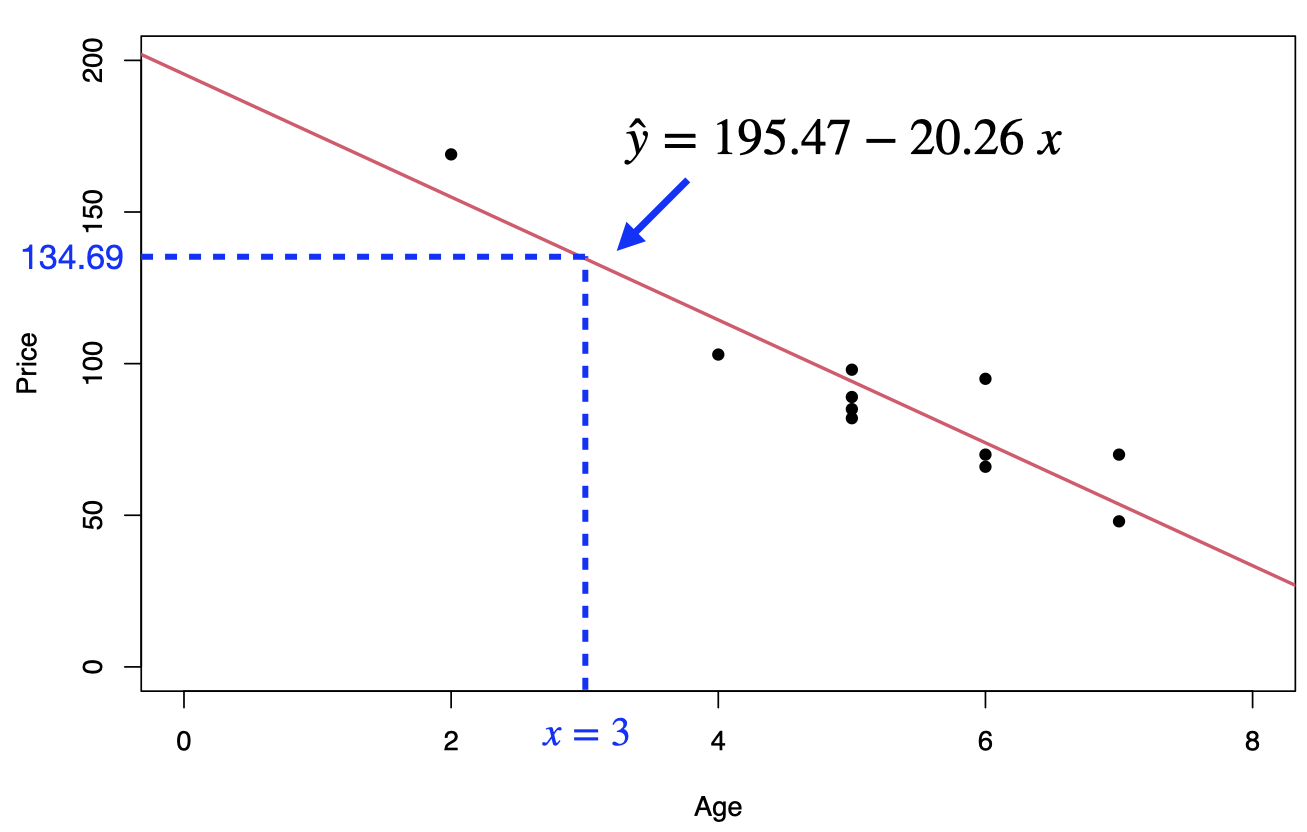
\includegraphics[width=0.4\linewidth,height=0.4\textheight]{figures/predex} \end{center}

A 95\% confidence interval for the mean price of all 3-year-old cars is
\[\hat{y}^*\pm t_{\alpha/2}\;\times se\sqrt{\frac{1}{n}+\frac{(x^*-\bar{x})^2}{S_{xx}}}\]
\[[195.47-20.26(3)]\pm 2.262\times12.58\sqrt{\frac{1}{11}+\frac{(3-5.273)^2}{(11-1)\times2.018}}\]
\[134.69\pm 16.76\] that is \[117.93<\mu^*<151.45\]

\textbf{Predict the price of a 3-year-old car, \(Y|x=3\)}:
\[\hat{y}^*=195.47-20.26 (3)= 134.69\]

A 95\% predictive interval for the price of a 3-year-old car is

\[\hat{y}^*\pm t_{\alpha/2}\;\times se\sqrt{1+\frac{1}{n}+\frac{(x^*-\bar{x})^2}{S_{xx}}}\]
\[[195.47-20.26(3)]\pm 2.262\times12.58\sqrt{1+\frac{1}{11}+\frac{(3-5.273)^2}{(11-1)*\times2.018}}\]
\[134.69\pm 33.025\] that is \[101.67<Y^*<167.72\]

where \(S_{xx}=\sum_{i=1}^{n} (x_i-\bar{x})^2=(n-1) Var(x)\).

\hypertarget{regression-in-r}{%
\subsection{Regression in R}\label{regression-in-r}}

\begin{Shaded}
\begin{Highlighting}[]
\CommentTok{\# Build linear model }
\NormalTok{Price}\OtherTok{\textless{}{-}}\FunctionTok{c}\NormalTok{(}\DecValTok{85}\NormalTok{, }\DecValTok{103}\NormalTok{,  }\DecValTok{70}\NormalTok{,  }\DecValTok{82}\NormalTok{,  }\DecValTok{89}\NormalTok{,  }\DecValTok{98}\NormalTok{,  }\DecValTok{66}\NormalTok{,  }\DecValTok{95}\NormalTok{, }\DecValTok{169}\NormalTok{,  }\DecValTok{70}\NormalTok{,  }\DecValTok{48}\NormalTok{)}
\NormalTok{Age}\OtherTok{\textless{}{-}} \FunctionTok{c}\NormalTok{(}\DecValTok{5}\NormalTok{, }\DecValTok{4}\NormalTok{, }\DecValTok{6}\NormalTok{, }\DecValTok{5}\NormalTok{, }\DecValTok{5}\NormalTok{, }\DecValTok{5}\NormalTok{, }\DecValTok{6}\NormalTok{, }\DecValTok{6}\NormalTok{, }\DecValTok{2}\NormalTok{, }\DecValTok{7}\NormalTok{, }\DecValTok{7}\NormalTok{)}
\NormalTok{carSales}\OtherTok{\textless{}{-}}\FunctionTok{data.frame}\NormalTok{(}\AttributeTok{Price=}\NormalTok{Price,}\AttributeTok{Age=}\NormalTok{Age)}

\NormalTok{reg }\OtherTok{\textless{}{-}} \FunctionTok{lm}\NormalTok{(Price}\SpecialCharTok{\textasciitilde{}}\NormalTok{Age,}\AttributeTok{data=}\NormalTok{carSales)}
\FunctionTok{summary}\NormalTok{(reg)}
\end{Highlighting}
\end{Shaded}

\begin{verbatim}
## 
## Call:
## lm(formula = Price ~ Age, data = carSales)
## 
## Residuals:
##     Min      1Q  Median      3Q     Max 
## -12.162  -8.531  -5.162   8.946  21.099 
## 
## Coefficients:
##             Estimate Std. Error t value Pr(>|t|)    
## (Intercept)   195.47      15.24  12.826 4.36e-07 ***
## Age           -20.26       2.80  -7.237 4.88e-05 ***
## ---
## Signif. codes:  0 '***' 0.001 '**' 0.01 '*' 0.05 '.' 0.1 ' ' 1
## 
## Residual standard error: 12.58 on 9 degrees of freedom
## Multiple R-squared:  0.8534, Adjusted R-squared:  0.8371 
## F-statistic: 52.38 on 1 and 9 DF,  p-value: 4.882e-05
\end{verbatim}

\begin{Shaded}
\begin{Highlighting}[]
\FunctionTok{mean}\NormalTok{(Age)}
\end{Highlighting}
\end{Shaded}

\begin{verbatim}
## [1] 5.272727
\end{verbatim}

\begin{Shaded}
\begin{Highlighting}[]
\FunctionTok{var}\NormalTok{(Age)}
\end{Highlighting}
\end{Shaded}

\begin{verbatim}
## [1] 2.018182
\end{verbatim}

\begin{Shaded}
\begin{Highlighting}[]
\FunctionTok{qt}\NormalTok{(}\FloatTok{0.975}\NormalTok{,}\DecValTok{9}\NormalTok{)}
\end{Highlighting}
\end{Shaded}

\begin{verbatim}
## [1] 2.262157
\end{verbatim}

\begin{Shaded}
\begin{Highlighting}[]
\NormalTok{newage}\OtherTok{\textless{}{-}} \FunctionTok{data.frame}\NormalTok{(}\AttributeTok{Age =} \DecValTok{3}\NormalTok{)}
\FunctionTok{predict}\NormalTok{(reg, }\AttributeTok{newdata =}\NormalTok{ newage, }\AttributeTok{interval =} \StringTok{"confidence"}\NormalTok{)}
\end{Highlighting}
\end{Shaded}

\begin{verbatim}
##        fit      lwr      upr
## 1 134.6847 117.9293 151.4401
\end{verbatim}

\begin{Shaded}
\begin{Highlighting}[]
\FunctionTok{predict}\NormalTok{(reg, }\AttributeTok{newdata =}\NormalTok{ newage, }\AttributeTok{interval =} \StringTok{"prediction"}\NormalTok{)}
\end{Highlighting}
\end{Shaded}

\begin{verbatim}
##        fit      lwr      upr
## 1 134.6847 101.6672 167.7022
\end{verbatim}

\(~\)

We can plot the confidence and prediction intervals as follows:

\begin{center}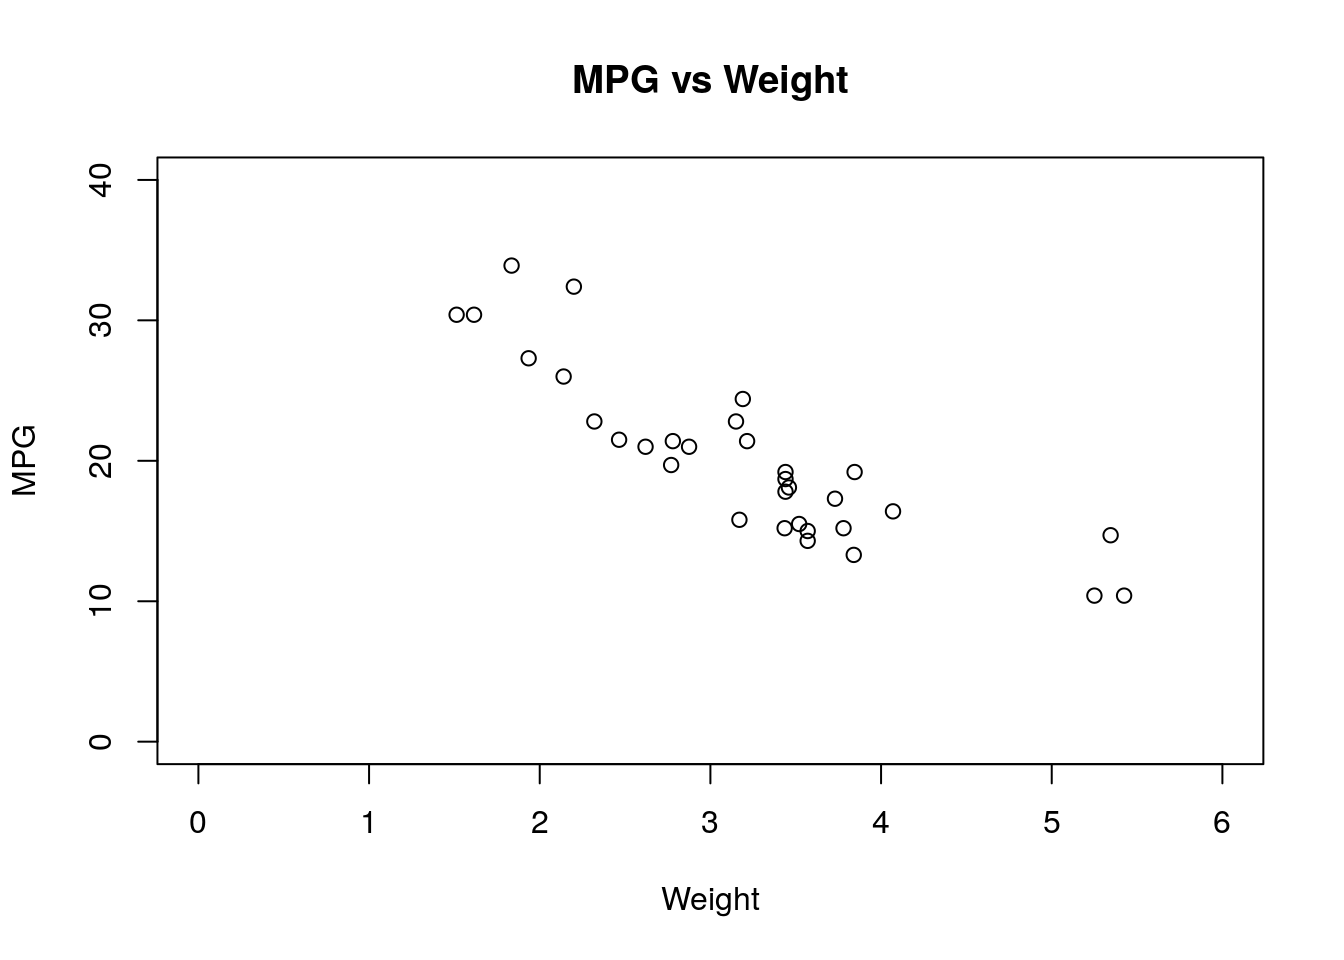
\includegraphics[width=0.8\linewidth,height=0.8\textheight]{4.3_Regression_Prediction_files/figure-latex/unnamed-chunk-4-1} \end{center}

\begin{center}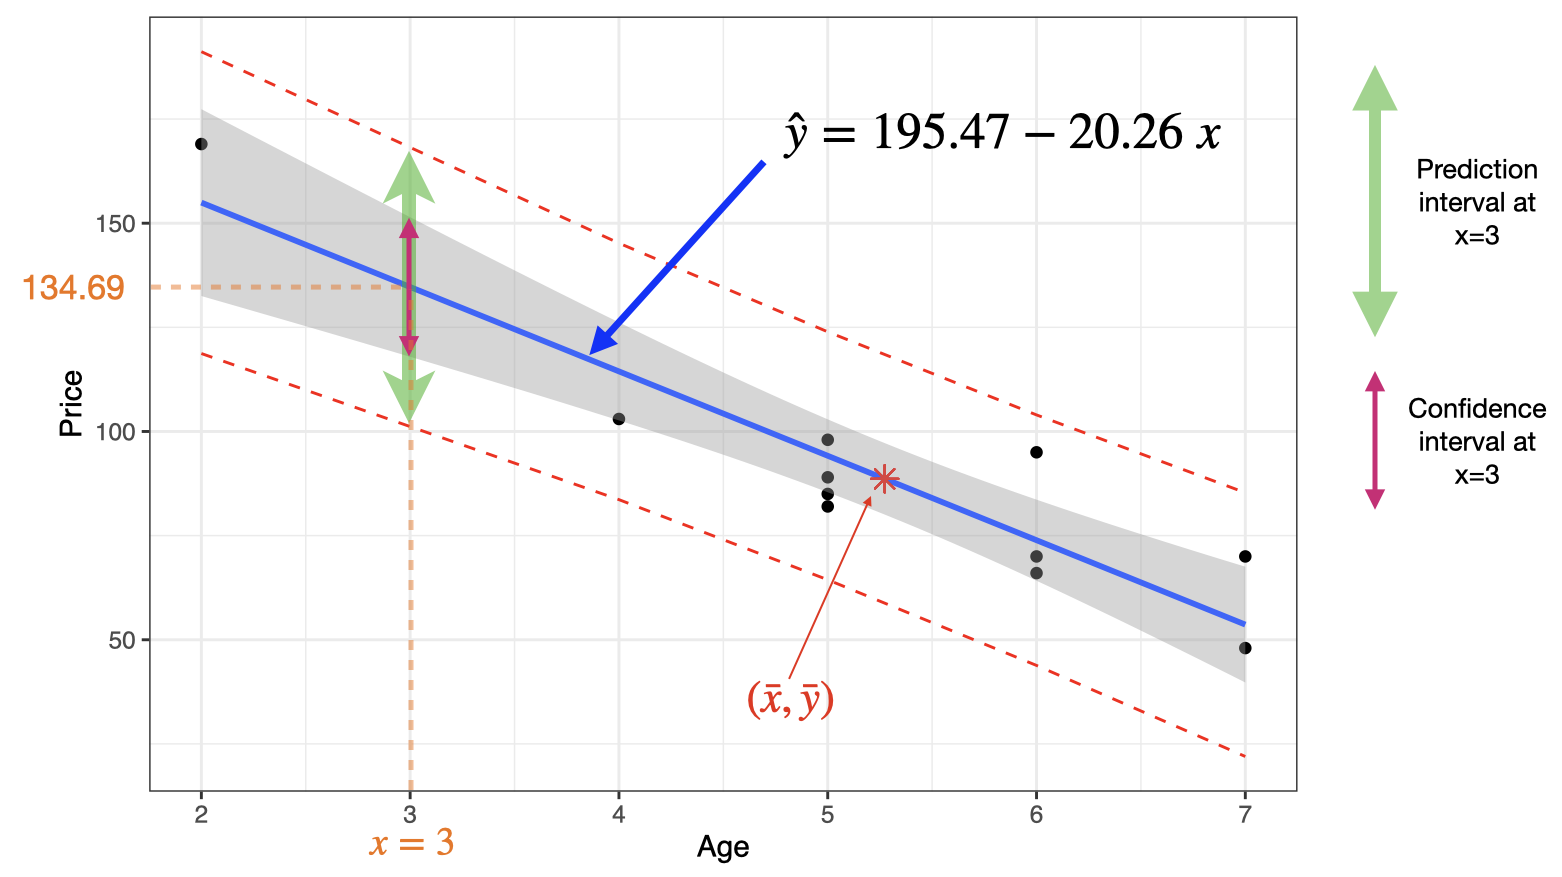
\includegraphics[width=0.8\linewidth,height=0.8\textheight]{figures/predex2} \end{center}

\end{document}
